\section{Comparing StableMoor $\ulow$ to IMU $\uhead$}
\label{apdx:ulow}

\def\ubt{\ensuremath{u_\mathrm{BT}}}

\begin{figure}[t]
  \centering
  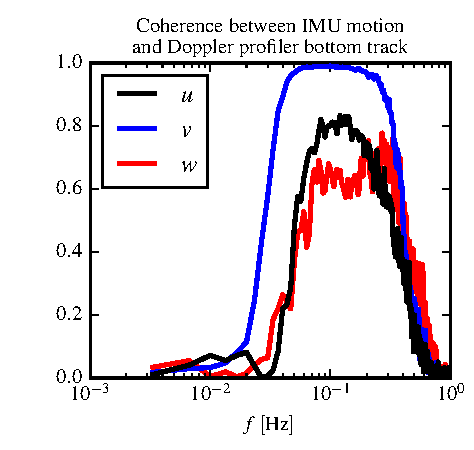
\includegraphics{BT_IMU_Coherence02}
  \caption{Coherence between IMU-measured motion of StableMoor buoy and ADP bottom track velocity for $1.0<\bar{U}<1.5$. The vertical dotted line indicates the 95\% confidence level for the 102 spectral windows in this estimate.}
  \label{fig:SM_coh}
\end{figure}

In order to better understand the IMU's signal-to-noise ratio, it is instructive to compare the motion of the StableMoor buoy from the ADP bottom track measurements, $\ubt$, to the IMU's estimates of ADP motion. To do this, we compute the IMU's estimate of ADP motion using equation \eqref{eqn:uhead}, and replacing $\ell^{*}$ with the vector that points from the IMU to the ADP head. We then linearly interpolated the ADP measurements onto the times of the ADV-IMU measurements.

The coherence between these two signals is high and statistically significant over 1.5 decades (from 0.03 to 0.8 Hz). The $v$ component has the highest coherence, 98\%, because this is the direction that has the most motion and therefore these estimates have a higher signal to noise ratio.  The $u$ and $w$ components have slightly lower coherence, 80\% and 65\%, respectively, which indicates the *convolved* signal to noise ratio of these measurements.

On the low-frequency side, our interpretation is that the signal to noise ratio of the IMU increases dramatically below 0.03 Hz, resulting in low coherence. On the high-frequency side Doppler-noise in the ADP measurements contaminates its estimates of motion, causing the decrease in coherence at 0.8 Hz. A comparison of the phase between these signals shows that there is no lag between the measurements (not shown).

These results help to inform the selection of zero-lag filters used to estimate $\ulow$ from $\ubt$. In particular, by selecting 0.2 Hz, we target the middle of the coherence peak between the two measurements. Furthermore, the rapid decrease in coherence below 0.03 Hz provides an objective measure of the performance of the frequency at which IMU measured velocity becomes unreliable in the flow conditions we observed. 



%%% Local Variables:
%%% mode: latex
%%% TeX-master: "Kilcher_etal_IMU-ADV"
%%% End:
